\documentclass[journal]{IEEEtran}
\usepackage[a5paper, margin=10mm]{geometry}
%\usepackage{lmodern} % Ensure lmodern is loaded for pdflatex
\usepackage{tfrupee} % Include tfrupee package


\setlength{\headheight}{1cm} % Set the height of the header box
\setlength{\headsep}{0mm}     % Set the distance between the header box and the top of the text


%\usepackage[a5paper, top=10mm, bottom=10mm, left=10mm, right=10mm]{geometry}

%
\usepackage{gvv-book}
\usepackage{gvv}
\setlength{\intextsep}{10pt} % Space between text and floats

\makeindex

\begin{document}
\bibliographystyle{IEEEtran}
\onecolumn
\newpage
\title{'2017-AE-'27-39'}
\author{AI24BTECH11004-Bheri Sai Likith Reddy}
\maketitle


\begin{enumerate}
       \item Let matrix \sbrak{A}=$\myvec{2&-6\\0&2}$. Then for any non-trivial vector \cbrak{x}=$\myvec{x_1\\x_2}$, which of the followning is true for the value of $K$=$\cbrak{x}^T\sbrak{A}\cbrak{x}$:
       \begin{enumerate}
           \item $K$ is always less thean zero 
           \item $K$ is always greater than zero
           \item $K$ is non-negative
           \item $K$ can be anything 
       \end{enumerate}
	\item consider the initial value problem:
        \begin{align*}
            \frac{d^2y}{dt^2}+4\frac{dy}{dt}+6y=f\brak{t}; y\brak{0}=2,\brak{\frac{dy}{dt}}_{t=0} =1
        \end{align*}
        If Y\brak{s} =$\int^\infty_0 y\brak{t}e^{-st}dt$ and $F\brak{s}=\int^\infty_0 f\brak{t}e^{-st}dt$ are the Laplace transforms of $y\brak{t}$ and $f\brak{t}$ ly, then $Y\brak{s}$ is given by:
               \begin{enumerate}
			        \begin{multicols}{2}  
		       \item $\frac{F\brak{s}}{\brak{s^2+4s+6}}$
		       \item $\frac{F\brak{s}+2s+9}{\brak{s^2+4s+6}}$
		       \item $\frac{F\brak{s}}{\brak{-s^2+4s+6}}$
		       \item $\frac{F\brak{s}-2s+9}{\brak{s^2+4s+6}}$
                    \end{multicols}   
	       \end{enumerate}	
       \item Let u\brak{x,t} denote the displacement of a point on a rod. The displacement satisfies the following w=equation of motion:
       \begin{align*}
           \frac{\partial^2u}{\partial t^2}-25\frac{\partial^2u}{\partial x^2}, 0<x<1
       \end{align*}
       with $u\brak{1,0}=0.01\sin \brak{10\pi x}, \frac{\partial u}{\partial t}\brak{x,0}=0; u\brak{0,t}=0, u\brak{1,t}$. The value of $u\brak{0.25,1}$ is \rule{1cm}{0.15mm} \brak{\text{in two decimal places}}.
	\item  The equation \begin{align*}
	    x\frac{d^2y}{dx^2}+5x\frac{dy}{dx}+4y=0
	\end{align*}
        has a soultion $y\brak{x}$ that is :
		\begin{enumerate}
			\item A polinomial in $x$
			\item Finite series in terms of non -integer fractional powers of $x$
			\item Consists of negative integer powers of xx and logarithmic function of $x$
	        \item Consists of exponential functions of $x$
        	\end{enumerate}
	\item Consider a straight wing with rectangular platform of aspect ratio $10$ and with a NACA $0012$ airfoil. The span effectiveness factor for this wing is $0.95$. Assume the flow to be incompressible and governed by thin airfoil theory. The lift coefficient of this wing, at an angle of attack of $6^\circ$, is \rule{1cm}{0.15mm} \brak{\text{in two decimal places}}.
	\item Consider an incompressible flow over a flat plate with the following approximation to the velocity profile:
 \begin{align*}
     \frac{u\brak{y}}{U}=\begin{cases}
         \frac{y}{\delta} \text{ for } y\leq \delta \\
1 \text{ for } y> \delta
     \end{cases}
 \end{align*}
 where $\delta$ is the boundary layer thickness and $U$ the free-stream speed. The normalized momentum thickness $\brak{\frac{\theta}{\delta}}$ for this profile is \rule{1cm}{0.15mm} \brak{\text{in two decimal places}}.
	\item An idealized velocity field is given by $\Vec{V}$ =$4tx\hat{i}-2t^2y\hat{j}+4xz\hat{k}$. At point \brak{-1,1,0} and at $t=1$, the magnitude of the material acceleration vector of the fluid element is \rule{1cm}{0.15mm}.
	\item A trace from the schlieren photograph of the flow around a corner reveals the edges of the expansion fan as shown below. The leading and trailing edges of the expansion fan make the angles as shown. Assuming $\gamma=1.4$, the angle of the expansion fan \brak{\text{in degrees}} is  \rule{1cm}{0.15mm} \brak{\text{in two decimal places}}.\\
    Pradtl Meyer function is given by 
    \begin{align*}
        v\brak{M}=\sqrt{\frac{\gamma +1}{\gamma +1}}\tan^{-1}\brak{\sqrt{\frac{\gamma -1}{\gamma +1}\brak{M^2-1}}}-\tan^{-1}\brak{\sqrt{M^2-1}}
    \end{align*}
    \begin{figure}[ht!]
        \centering
        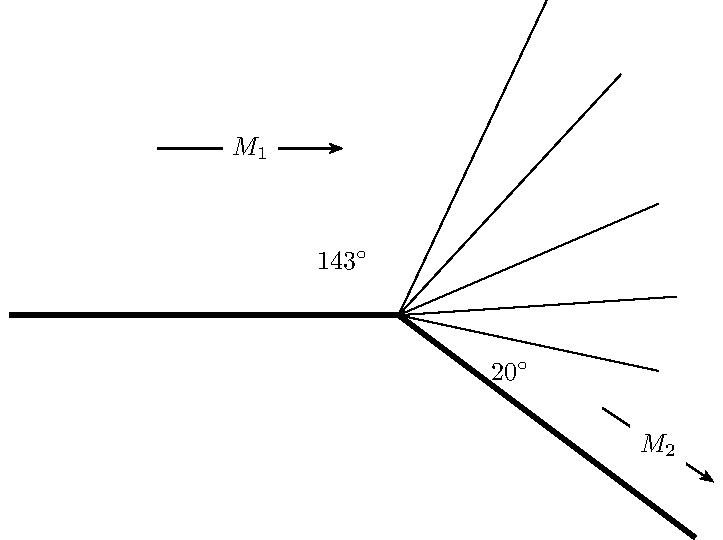
\includegraphics[width=0.5\linewidth]{fig/fig1.pdf}
    \end{figure}
	\item A strong normal shock wave, with a pressure ratio of $29$ across it, is traveling into stationary air $\brak{\gamma = 1.4}$ at $T=280K$ in a straight duct \brak{see figure}. The magnitude of the velocity of the air induced behind the shock wave is \rule{1cm}{0.15mm} m/s. \brak{\text{in two decimal places}}.
    (Gas constant $=287J/kg.K$; Shock wave relations:
    \begin{align*}
        \text{Pressure ratio: } \frac{p_1}{p_2}=1+\frac{2\gamma}{\gamma+1}\brak{M^2-1}; \text{Density ratio: } \frac{\rho_2}{\rho_1}=\frac{\brak{\gamma+1}M^2}{\gamma-1M^2+2}
    \end{align*})
		\newpage
  \begin{figure}[ht!]
        \centering
        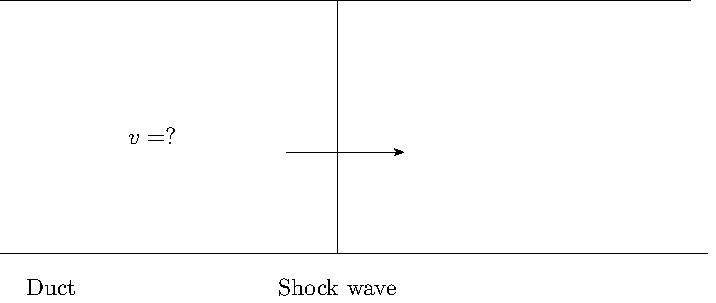
\includegraphics[width=0.5\linewidth]{fig/fig2.pdf}
    \end{figure}
	\item In the figure below,  water exits from  a nozzle into atmospheric pressure of $101 kPa$. If the exit velocity id $V_2=8m/s$ and friction is neglected,  the magnitude of the axial force on the flange at location $1$ required to keep the nozzle attached to the pipe is \rule{1cm}{0.15mm}N \brak{\text{in two decimal places}}.
  \begin{figure}[ht!]
        \centering
        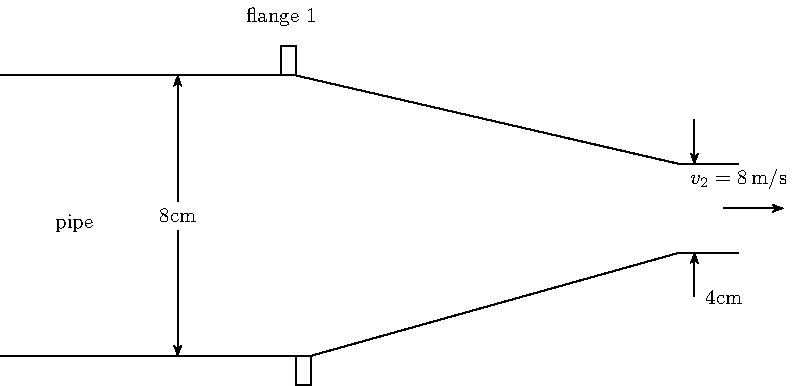
\includegraphics[width=0.5\linewidth]{fig/fig3.pdf}
    \end{figure}
	\item  A football meant to be thrown at $100km/h$ in sea level air $\brak{\rho = 1.22 kg/m^3,\mu =1.78x10^{-5}N-s/m^2}$, is to be tested using a one-quarter scale model in a water tunnel $\brak{\rho =1000kg/m^3,\mu=10^{-3}N-s/m^2}$. For dynamic similarity, the ratio of the model force to the prototype force is \rule{1cm}{0.15mm} \brak{\text{in two decimal places}}.
	\item An aircraft model was tested in a low speed wind-tunnel \brak{\text{Reynolds number =}2x10^6\text{ based on wing mean chord}. } The variation of pitching moment coefficient $\brak{C_m}$ with angle of attack $\brak{\alpha}$ for two elevator deflections $\brak{\delta_e}$ as recorded during this test is presented below.
 \begin{figure}[ht!]
        \centering
        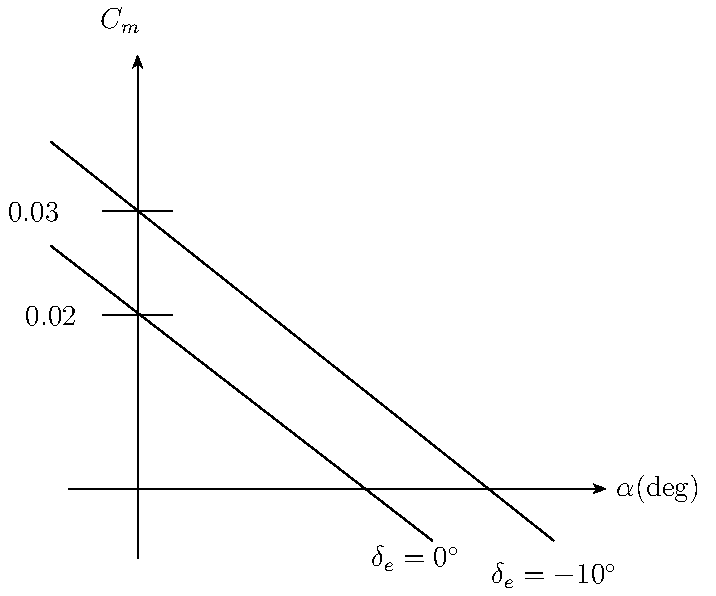
\includegraphics[width=0.5\linewidth]{fig/fig4.pdf}
    \end{figure}
 Based on the result presentes in the figure above, the value of elevator control power $\brak{C_{m\delta e}}$ in per radian will be \rule{1cm}{0.15mm} \brak{\text{in two decimal places}}.
    \item A pilot was flying a single-engine propeller aircraft and maintaining a steady level flight at a lift coefficient, $C_L=0.5$ at an altitude of $500m$. Due to some emergency, at the same altitude $\brak{500m}$, the pilot had to fully deploy the landing gear. If the pilot wants to maintain steady level flight at the same $CF_L =0.5$ and at the same altitude, which of the following control actions should the pilot undertake:
    \begin{enumerate}
        \item Move the elevator up, and decrease the throttle
        \item Move the elevator up, and increase the throttle 
        \item Move the elevator down, and decrease the throttle 
        \item Move the elevator down, and increase the throttle
        
    \end{enumerate}
\end{enumerate}	
\end{document}
